
\subsection{Information Centric Networking}
Information-Centric Networking (ICN) is a communication paradigm for the future Internet that is based on \textit{named data} instead of \textit{named hosts}. It represents an evolution of the Internet from todays host-centric networking, in particular IP networking, towards an information-centric approach.\\\\
There are several different approaches of implementing the ICN paradigm, but there are fundamental ideas that they all follow regardless which implementation is used. This section will continue describing the general ideas. However, the thesis overall will only consider the \textit{Content Centric networking} approach described more in depth at section [ref till CCN].\\\\
Some of the main features in the ICN are the possibility of in-network storage for caching data, multiparty communication through replication, decoupling senders and receivers, and that data is named\cite{Ahlgren2012}. In information-centric networks, an information request may not only be satisfied by locating the original information source, it is possible for any of the in-network caches to reply to the request with the desired data if they hold any copies of it. After a request is sent from a user, it is the responsibility of the network to locate the best source that can provide the information. Due to the fact that information/data is named, addressed and matched independently from its location, the data may be located anywhere in the network[icn research][18][19]. Hence the argument that the ICN approach decouple the information from its source.\\\\




\subsubsection{Content-Centric Networking}



%\begin{itemize}
%\item motivation, one type of ICN architecture. 
%\end{itemize}
The CCN communication \cite{Jacobson2009} is driven by consumers of data. There are two types of message in CCN, \textit{Interest} and \textit{Data}. A consumer issues an \textit{Interest} message to request an information object on the network. Any node that recieved the interest and containing the requested information, will respond by sending the \textit{Data} back to the \textit{Interest} issuer. A \textit{Data} message is only sent in response to an \textit{Interest} message, upon response, the interest message will cease to exist in the network.
\\\\
A key feature of CCN is that the content names are hierarchical. This allows routing information to be aggregated which in turn is critical in order to scale the network. The content name can be simila to URLs, for example a valid content name could be \textit{/sics.se/kista/floor/six/sensor/two/temperature}. However, there is neither a strict need for them to be human-readable nor tobe a URL. The prefix \textit{/sics.se/kista/floor/six/sensor/two/} could easily be exchanged to become either a hash value or just an integer, say \textit{2} (representing the sensor two), whereby the same data could be accessable by the name \textit{/2/temperature}.
\\\\
It is to be considered an interest hit when any part of the interest name equals the named prefix of the data, for example is it possible that \textit{/2/temperature} could be match by \textit{/2/temperature/sequence$\_$1}. If the data is produced periodically with sequence numbering, a consumer can `follow' the data by the same manner once it has a starting point. Another advantage with periodically and sequencing, is that it provide the possibility to ask for data that has not yet been produced. A consumer could potentially issue an \textit{interest} request a short time before the \textit{data} has been produced, which would firstly get the data directly to the user and secondly minimise the latency on the network[ref to bengt2](No performance evaluation of this has been done to date, the thesis will try to answer the feasability of this.). 
\\\\
Even though there are a lot of similiarities to regular routers IP, there are a lot of differences between a CCN router and a regular IP router.
Every Content Router (CR) maintain three main data structures: The Forwarding Information Base (FIB), the Pending Interest Table (PIT) and the Content Store (CS).
\\\\
The FIB is used to map information to on which output interface a Interest message should be forwarded to in order to reach its content. It is very similar to a regular FIB in a IP router, with the major difference that the CCN FIB allows lists of outgoing interfaces instead if just a single entry per object.
\\\\
The PIT maintain a table for all incoming \textit{interests} request recieved by the CR, their current state and a mapping to which face they came from[Bengt]. When the data message for a particular \textit{interest} arrives to a CR, the data message will be forwarded back on a reverse path, towards the face that exist in the corresponding PIT entry. After the data message has been forwarded towards the requester, its entry in the PIT will be erased. Whenever an entry is dropped or lost, for instance due to timeouts, it is up to the consumer to issue a new interest request.\
\\\\
The CS act as a local cache for information objects that has passed through the CR.
\\\\
With the use of the CRs, CCN has great support for data caching. As stated earlier, once a \textit{interest} is receievd, the CR will look through its CS in order to find matching data. Once the data is on the reverse path to the consumer, it will be put in the CS for a limited period of time for futhre use. Although there are several benefits using the cache in a distributed network system, it should be pointed out that this is not a long-term storage since a router can not hold infinite number of data. Nor is it useful for data objects that are requested at most once, since the benefits only occur when the data is requested a second time \cite{Ahlgreniot}\cite{Ahlgren2012}. %[Ahlgren2][surveyiot].
\\\\
An example of CCN in action is illustraded in figure \ref{fig:CCN-architecture}. Here, a consumer wants to retrive the indoor temperature data from the producer.
Consumer1 sends an \textit{interest} for data \textit{/temp/indoor} towards CR1. When it arrives, CR1 looks for data in its CS that matches the requested prefix of the interest. Since there is no match in the CS, the router performs a lookup on the longest prefix that matches its FIB in order to decide where to forward the incoming interest. When the match in the FIB is found, the router inserts the interest, with the incoming interface, into the PIT.\\
The same procedure happens for CR2 and the interest will be put in the PIT and forwarded to the producer. When the \textit{interest} reaches the producer, it matches the name of the \textit{data} and thereby the \textit{interest} message is discarded and the \textit{data} is sent back towards CR2. When the data is received, CR2 stores the data in the cache. Thereafter it performs a longest-prefix match in its PIT to get which interface it should respond to. In this case, it will respond to CR1 and the same forward back procedure will occur at CR1 until the data reaches the consumer.\\
When Consumer2 later on wants the same content, it sends an \textit{interest} to CR1 and will retreive the data directly from its cache and thereby reducing the network traffic.



\begin{figure}
	%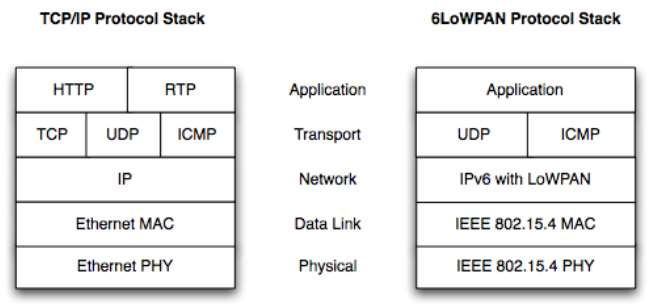
\includegraphics[width=\textwidth]{figures/ip-6lowpan-stack.jpg}
	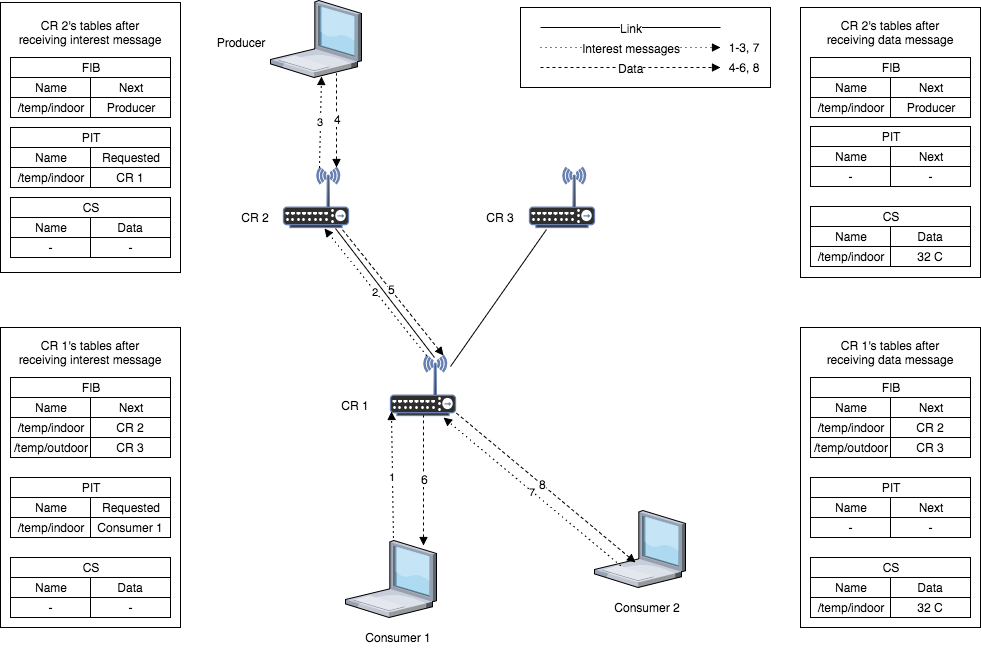
\includegraphics[width=\textwidth]{figures/CCN-architecture.png}
	%\caption{Star topology structure on the left, Peer-to-peer on the right. write where it is taken from?}
	%\caption{Simplified OSI model, an example TCP/IP stack and an illustration of the 6LowPAN protocol stacks, copied from \cite{rfc4944}}
	\caption{The CCN architecture builed up by content routers (CR), forwarding information base (FIB), pending interest table (PIT) and content store (CS), inspired by [ref survey ICN]}
	\label{fig:CCN-architecture}
\end{figure}



\subsubsection{Using ICN for IoT}
The usage of IoT devices most often implies an information centric pattern. In many scenarios, the main goal is the data and services and it is less important to communicate with a specific device \cite{Ahlgreniot}. Where users and/or devices rather consume content, generated by an IoT device, through the network than connecting directly to a specific device or host. Therefore one could argue that naming the data is more important than naming the devices.\\
Depending on topology structure of the IoT network, the caching mechanisms ICN provides could help constrained IoT devices to avoid unnecessary transmissions when distributing its data into multiple places. Storing cached data in the network could also potentially save energy and network bandwidth of an IoT device.

% There are several reasons why it is better to use an ICN approach in the IoT domain. Everything always depends on application and usage, but there are some pros and cons using ICN in the IoT domain.
% 
% \begin{itemize}
% 	\item + naming of data
% 	\item + distributed caching
% 	\item + Decoupling between publisher and consumer
% 	\item + Sending request for the future.
% 	\item advantages of using ICN in IoT domain.
% 	\item disadvantages
% 	Even though the major advantage of using named data in IoT, it comes with some concerns. How to create and format efficient names suitable for huge numbers.
% \end{itemize}




\subsubsection{CCN-lite}
CCN-lite is a lightweight, functionally implementation of CCN \cite{CCN-LITE}. There are several platforms that are supported such as UNIX, Linux, Android, Arduino and several other. It uses a small code base of C, less than 2000 lines of code, in order to implement the CCN functionality. CCN-lite runs over UDP and Ethernet, and support packet fragmentation.
\\




















